\begin{frame}
\frametitle{Introduction}

\vspace{2mm}

% Based on the following works:
{
\small
\begin{itemize}\setlength\itemsep{0.75em}
    \item[\ding{112}] [L\textbf{O}SW24]
    \textit{Neural network learns low-dimensional polynomials near the information-theoretic limit}. 
    \item[\ding{112}] [\textbf{O}SSW24]
    \textit{Learning sum of diverse features: computational hardness and efficient gradient-based training for ridge combinations}.
\end{itemize}
} 

\vspace{4mm} 
  
\begin{figure}[t]
\centering
\begin{minipage}[t]{0.23\linewidth}
\centering
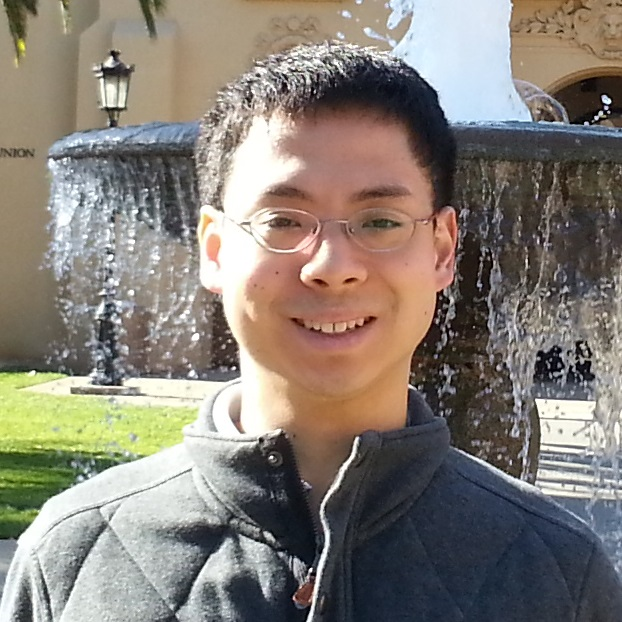
\includegraphics[height=0.9\textwidth]{profile_pic/JL} \\ \vspace{-0.1cm}
{\footnotesize Jason D.~Lee}
\end{minipage}
\begin{minipage}[t]{0.23\linewidth}
\centering    
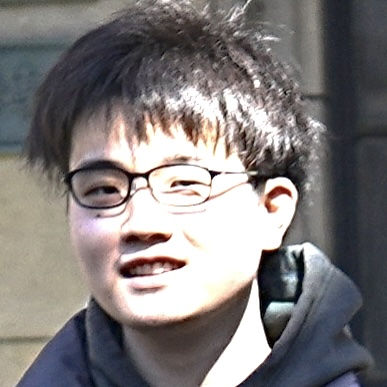
\includegraphics[height=0.9\textwidth]{profile_pic/YS} \\ \vspace{-0.1cm}
{\footnotesize Yujin Song}
\end{minipage}
\begin{minipage}[t]{0.23\linewidth}
\centering    
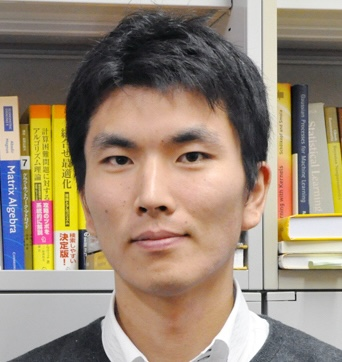
\includegraphics[height=0.9\textwidth]{profile_pic/TS2} \\ \vspace{-0.1cm}
{\footnotesize Taiji Suzuki}
\end{minipage}\vspace{1mm} 
\begin{minipage}[t]{0.23\linewidth} 
\centering    
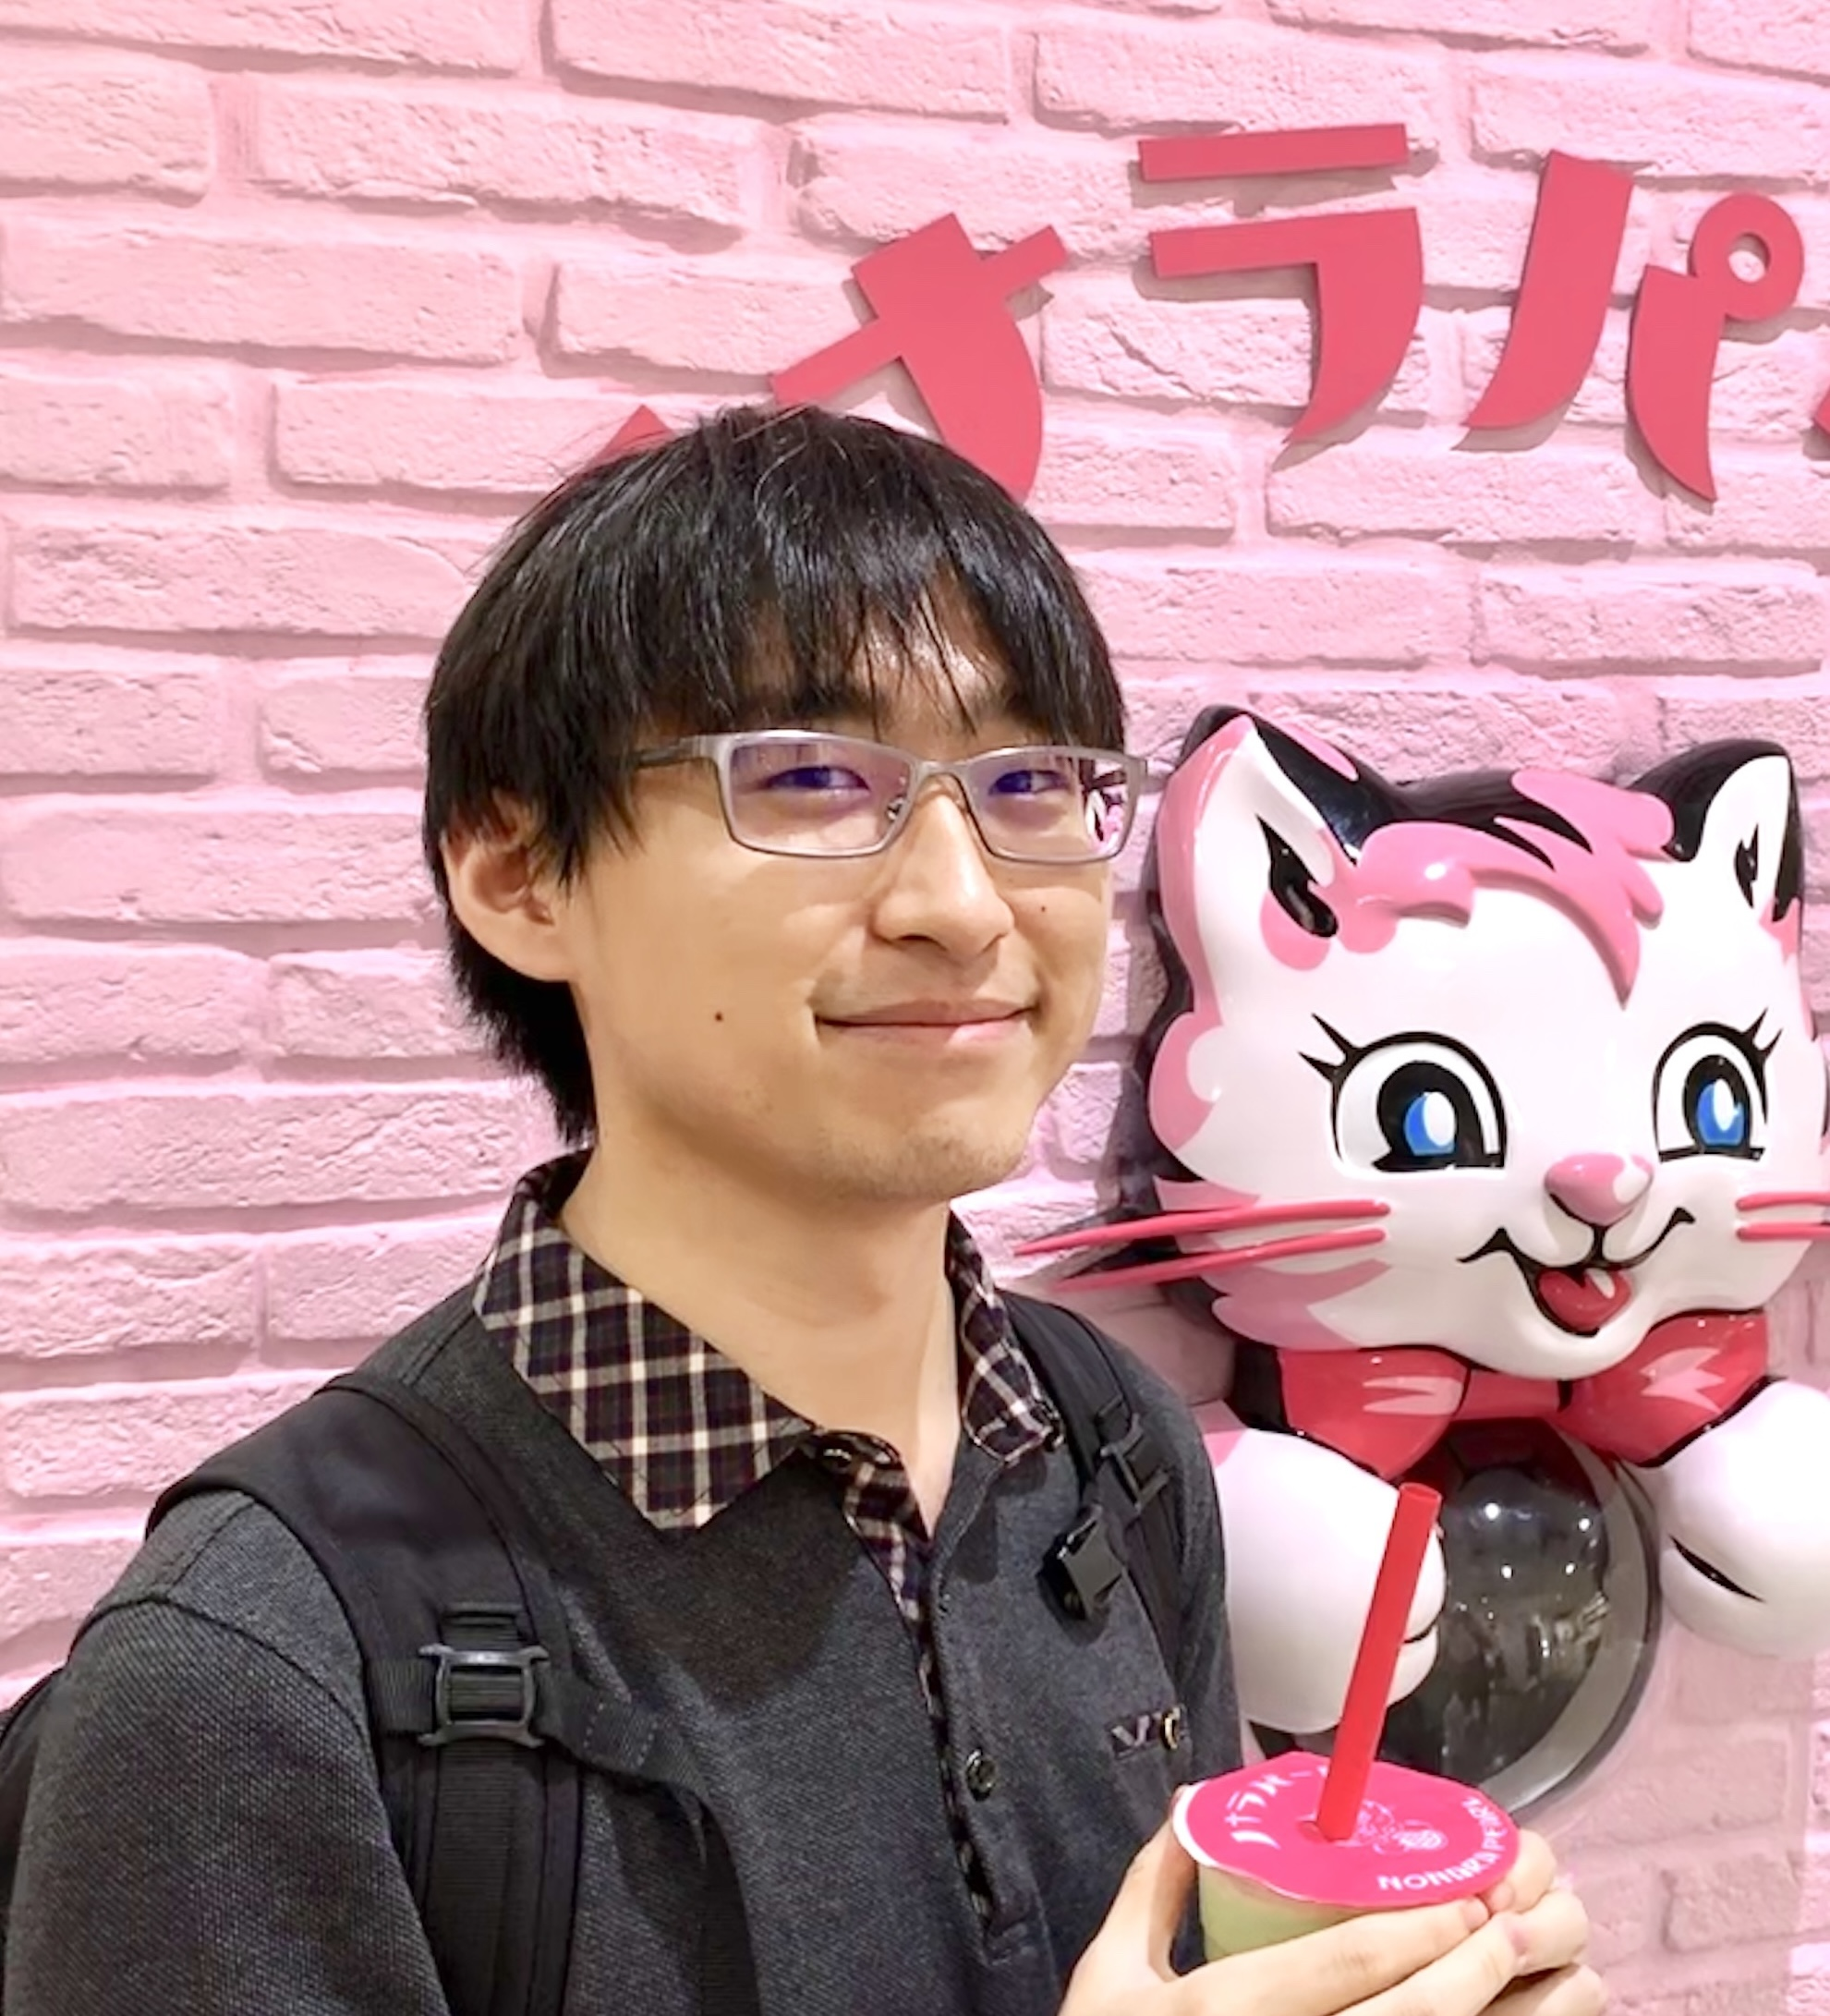
\includegraphics[height=0.9\textwidth]{profile_pic/DW} \\ \vspace{-0.1cm}
{\footnotesize Denny Wu}
\end{minipage}
% \begin{minipage}[t]{0.23\linewidth}
% \centering    
% 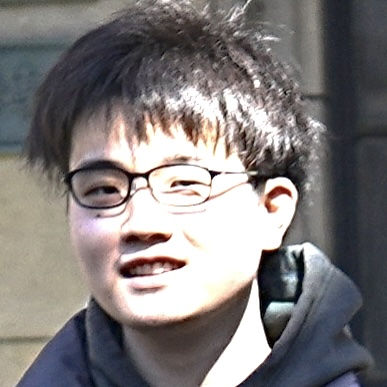
\includegraphics[height=0.9\textwidth]{profile_pic/YS} \\ \vspace{-0.1cm}
% {\footnotesize Yujin Song}
% \end{minipage}\vspace{1mm} 
% \begin{minipage}[t]{0.23\linewidth} 
% \centering    
% 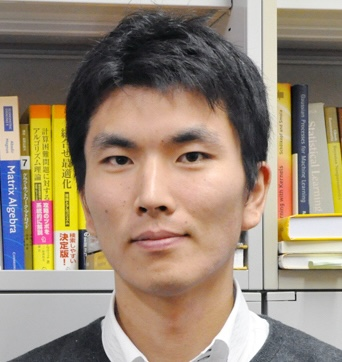
\includegraphics[height=0.9\textwidth]{profile_pic/TS2} \\ \vspace{-0.1cm}
% {\footnotesize Taiji Suzuki}
% \end{minipage}
\end{figure}    
  

\end{frame}